\section{Related Work}%
\label{sec:state}

In dynamic environments, global planning methods are not sufficient
due to low planning frequencies. Thus, local motion generation methods, like
the one presented in this work are employed. These methods typically
require guidance to avoid local minima and thus effectively solve planning problems.

\subsection{Task constrained global motion planning}%
\label{sub:state_global}

Motion planning problems are usually defined by goals in arbitrary task spaces,
such as the 3D Euclidean space or end-effector poses. In this
context, tasks can be regarded as constraints to the motion planning problem.
Conventional approaches to motion planning rely on inverse kinematics to
transform task constraints into sets of configurations. The resulting global
motion planning problem is then often solved using sampling-based methods
\cite{Rickert2014}.

Sampling-based motion planners generate random configurations
until a valid path between an initial
configuration and a set of goal configurations is found
\cite{Karaman2011}. Several methods have been proposed to directly
integrate task constraints into the sampling phase. 
\cite{Stilman2010} proposed a
method to iteratively push a random sample to the manifold adhering to the task constraint.
The notion of
task constraints was later extended to task space regions to define soft constraints for
individual task components~\cite{Berenson2011}.
\cite{Kingston2019} proposed scalar-valued functions to represent task
constraints for sampling-based planning.
As all of the above-mentioned methods rely on implicitly constrained sampling
in the joint space, they exhibit high computational time, which is especially
harmful to real-world applications \cite{Qureshi2020}
and require local motion generation methods for path following
and execution in dynamic environments
\cite{Brito2019}.
In the next
subsection, recent developments in local motion planning are summarized.

\subsection{Receding-horizon trajectory optimization}%
\label{sub:state_local}

Methods formulating motion generation as an optimization problem with a finite
discrete time horizon are known under the name of receding-horizon trajectory
optimization. In line with most literature in robotics, we will refer to such
methods as \ac{mpc}.
Generally, several objectives are encoded in the scalar cost function, dynamics
are formulated as equality constraints and inequality constraints ensure
collision avoidance and joint limit avoidance. The dynamics for this problem can
include the full dynamics model or simple integrating schemes \cite{Hewing2020}.
By explicitly solving the constrained optimization problem, this approach yields
formal guarantees on stability. Stability for \ac{mpc} is proven by formulating
an appropriate Lyapunov function and showing that the finite time-horizon
formulation with an appropriate terminal cost results in the same stability as
the corresponding infinite time-horizon formulation
\cite{l1,l4,keerthi1988optimal}. \ac{mpc} has been applied to various robotic
systems in dynamic environments, such as drones \cite{Tordesillas2019}, mobile
robots \cite{Brito2019}, and mobile manipulators
\cite{Avanzini2015,Avanzini2018}. Despite these results, formal stability
guarantees in such environments are challenging as appropriate terminal cost
functions are often not computable or too conservative. Besides, the
computational costs scale with the degrees of freedom restricting real-time
applicability to simple dynamics and environment models \cite{Spahn2021}.

Some \ac{mpc} formulations are non-linear and can be analyzed
using methods from non-linear control. When analyzing non-linear control
system, Riemannian energies lead to more detailed stability results than
Lyapunov functions. By investigating the variation around the generated
trajectory and its contracting towards the desired trajectory, some control
designs show exponential stabilizing properties \cite{l2}. These
findings have been applied to tracking control problems \cite{l3}.

\subsection{Riemannian motion policies and fabrics}%
\label{sub:riemannian_motion_policies_and_fabrics}

Based on the findings of contracting metrics for non-linear
control design \cite{l2,l3}, geometric control approaches design the motion
generation such that convergence is inherent to the problem formulation
rather than imposing them on the solution process. Practically, individual
constraints to the motion planning problem shape the optimization manifold
so that the solution is accessible through the solution of simple differential
equation. An example for shaping the optimization
manifold is seen in \cref{fig:spec_combination}.

%
\begin{figure}[h]
  \centering
  \begin{subfigure}{0.33\linewidth}
    \centering
    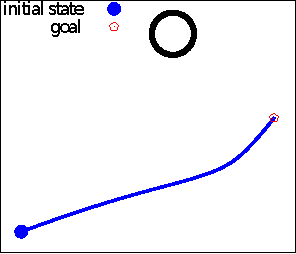
\includegraphics[width=0.9\textwidth]{state/trajectory_obst2}
    \caption{}
    \label{subfig:trajectory_obst1}
  \end{subfigure}%
  \begin{subfigure}{0.33\linewidth}
    \centering
    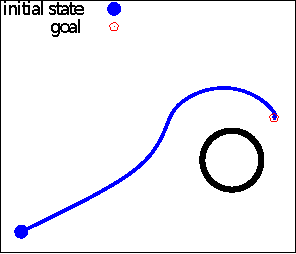
\includegraphics[width=0.9\textwidth]{state/trajectory_obst1}
    \caption{}
    \label{subfig:trajectory_obst2}
  \end{subfigure}%
  \begin{subfigure}{0.33\linewidth}
    \centering
    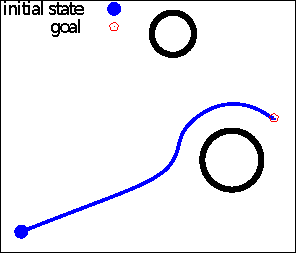
\includegraphics[width=0.9\textwidth]{state/trajectory_both_obstacles}
    \caption{}
    \label{subfig:trajectory_both_obstacles}
  \end{subfigure}
  \caption{
    Combining different avoidance behaviors using optimization fabrics. The
    components defining collision avoidance with single obstacles (a,b) are
    combined in (c). Obstacles are shown in black. Trajectories of the point
    robot are shown in blue.
  }
  \label{fig:spec_combination}
\end{figure}
%
Realizing this concept, Riemannian motion policies (RMPs) represent a
natural way of combining multiple policies into one joined policy.
RMPs define individual sub-tasks of the motion planning as
differential equations (\textit{spectral semi sprays} or
\textit{specs} for short) of second order and propose the
\textit{pullback} and \textit{summation} operators to combine multiple policies
in the configuration space. As subtasks can be defined in arbitrary manifolds
of the configuration space, RMP generalize operational space
control~\cite{Khatib1987}. The resulting behavior of RMP was reported to be
intuitive while keeping computational costs low~\cite{Ratliff2018}. The concept
of RMP was used in~\changed{\cite{Cheng2018,Cheng2020}} to form RMP-Flow, a motion
planning algorithm that is shown to be conditionally stable and invariant
across robots. In RMP-Flow, individual tasks are represented as a pair of
a motion policy and a corresponding metric defining the importance of
individual directions. An RMP adaptation was proposed for non-holonomic robots
in~\cite{Meng2019}. By incorporating the kinematic constraint into the root
equation of the RMP, the computed policy is applicable to non-holonomic robots.
Besides, that work proposed a neural net to learn the collision avoidance task
components. 

Although RMPs have proven to be a powerful tool for
motion generation, it was reported to require intuition and experience
during tuning~\cite{Ratliff2020}. Optimization fabrics with Finsler structures
as metric generators simplify the motion design as the conditions for stability
and convergence are inherent to the definition of Finsler
structures~\cite{Ratliff2020,Ratliff2021}. Opposed to RMPs, where the metric is
typically user-defined, fabrics derive Finsler metrics from artificial
energies, similar to approaches from control design, \cite{l2,l3}, using the
Euler-Lagrange-Equation from geometric mechanics. Although fabrics generalize
the concept of RMPs and make it accessible to a broader audience by
decreasing the intuition and expertise required, they have not yet been applied
to a wide range of robots. 

The reason for this lack of application of fabrics is twofold. First, all the
above mentioned methods are reactive and highly local methods, thus making them
prone to local minima \cite{Bhardwaj2021}. As RMPs and optimization
fabrics do not incorporate path following, integration of global
planning to overcome local minima is not possible to this date. Second, fabrics
and RMP do not make use of velocity estimates of obstacles but rely purely on
their high reactivity in dynamic environments. As for other trajectory
optimization techniques, motion estimates could benefit fabrics (and RMP) to
result in even smoother motion and allow applications in such environments. 

In this paper, we address these issues by proposing time parameterized
differential maps to form \acl{df}. This generalization integrates
path following and velocity estimates of moving
obstacles. Together with the extension to non-holonomic robots, our method
allows to deploy the promising theory of optimization fabrics to mobile
manipulators, operating in dynamic environments.

